\documentclass[12pt,a4paper]{article}

\usepackage[utf8]{inputenc}
\usepackage[T2A]{fontenc}
\usepackage[russian]{babel}
\usepackage{amsmath,amssymb}
\usepackage{graphicx}
\usepackage{booktabs}
\usepackage{multirow}
\usepackage{geometry}
\geometry{top=2cm,bottom=2cm,left=2.5cm,right=1.5cm}
\usepackage{float}

\title{\textbf{Лабораторная работа 1.1.4}\\
Изучение статистических закономерностей на примере измерения фона космического излучения}

\author{
    Студент \underline{Шеховцов Василий Максимович}\\
    Группа \underline{Б03-601}\\
    Преподаватель \underline{Ивлев Д.А.}
}
\date{Московский Физико-технический институт\\
(национальный исследовательский университет)\\
22 сентября 2026 г.}

\begin{document}
\maketitle

\section*{Цель работы}

На примере статистики регистрации фоновых космических частиц изучить статистические закономерности однородного во времени случайного процесса; проверить возможность описания исследуемого процесса статистическими законами Пуассона и Гаусса; измерить среднее число регистрируемых космических лучей в секунду и определить погрешность результата.

\section*{Оборудование}

\begin{itemize}
    \item Счётчик Гейгера--Мюллера (СТС-6);
    \item блок питания;
    \item компьютер с интерфейсом связи со счётчиком.
\end{itemize}

\section*{1. Теоретические сведения}

Радиоактивным излучением называют потоки частиц (протонов, электронов и позитронов, альфа-частиц, нейтронов и т.п.) или электромагнитных волн, способных вызывать ионизацию вещества. Основными источниками радиации являются космические лучи и распад радиоактивных веществ. Основную часть фона обычно составляет космическое излучение, которое исходно состоит из протонов ($\approx$85\%), альфа-частиц ($\approx$10\%), ядер более тяжёлых элементов ($<$5\%) и электронов и позитронов ($\approx$1\%). При взаимодействии этих лучей с атмосферой Земли рождается разнообразное множество нестабильных частиц (мюоны, пи-мезоны и др.).

\subsection*{Устройство счётчика Гейгера--Мюллера}

Счётчик Гейгера--Мюллера представляет собой наполненный газом металлический цилиндр с двумя электродами. Одним из электродов (катодом) служит сам корпус, другим (анодом) — тонкая нить, натянутая вдоль оси цилиндра. Необходимое напряжение (400~В) подаётся на счётчик от блока питания.

Радиоактивное излучение ионизует молекулы газа, которым наполнен счётчик, а также выбивает электроны из его стенок. Образовавшиеся электроны, ускоряясь в сильном электрическом поле между электродами счётчика, соударяются с молекулами газа, выбивая из них новые вторичные электроны. В результате образуется лавина электронов, и через счётчик протекает кратковременный импульс тока. Этот импульс регистрируется электрической цепью установки, оцифровывается и через USB-интерфейс передаётся на компьютер.

\subsection*{Статистическая обработка данных: базовые сведения}

Результат любого физического измерения содержит погрешности. Частным случаем случайных погрешностей являются статистические погрешности, вызываемые случайными колебаниями (флуктуациями) самой измеряемой величины. К числу таких флуктуирующих величин относится и интенсивность космического излучения.

Пусть при некотором измерении за время $\tau$ зарегистрировано $n$ космических частиц. Из этого не следует, что в любые следующие $\tau$ секунд будет регистрироваться то же число частиц: в силу случайных причин можно получить любое другое значение, не слишком сильно отличающееся от $n$. Поэтому физический смысл имеет не результат отдельного измерения, а совокупность множества результатов и её усреднённые характеристики.

Выборочное среднее значение числа регистрируемых частиц:
\begin{equation}
    \langle n\rangle \equiv \frac{1}{N}\sum_{i=1}^{N} n_i.
    \label{eq:mean}
\end{equation}

Мера флуктуаций значений $n_i$ около среднего — среднеквадратичное (стандартное) отклонение, определяемое через выборочную дисперсию:
\begin{equation}
    \sigma_n^2 \equiv \frac{1}{N}\sum_{i=1}^{N}(n_i - \langle n\rangle)^2.
    \label{eq:variance}
\end{equation}

Погрешность среднего значения при независимых измерениях связана со стандартным отклонением отдельного измерения формулой
\begin{equation}
    \sigma_{\langle n\rangle} = \frac{\sigma_n}{\sqrt{N}}.
    \label{eq:mean_error}
\end{equation}

Истинное среднее значение $\bar n$ с высокой вероятностью лежит в интервале
\begin{equation}
    \bar n = \langle n\rangle \pm \sigma_{\langle n\rangle}.
    \label{eq:final_result}
\end{equation}

\subsection*{Распределение Пуассона}

Если случайные события (регистрация частиц) однородны во времени, а каждое последующее событие не зависит от предыдущих, такой процесс называется пуассоновским. Вероятность зарегистрировать $n$ частиц описывается распределением Пуассона:
\begin{equation}
    w_n = \frac{\bar n^{\,n}}{n!}\,e^{-\bar n},
    \label{eq:poisson}
\end{equation}
где $\bar n$ — единственный параметр распределения, совпадающий со средним числом частиц.

Наиболее характерное свойство распределения Пуассона — равенство среднеквадратичного отклонения корню из среднего значения:
\begin{equation}
    \sigma_n \approx \sqrt{\langle n\rangle}.
    \label{eq:poisson_property}
\end{equation}

При $\bar n \gtrsim 10$ распределение Пуассона приближается к нормальному распределению (распределению Гаусса), для которого известно, что отдельное измерение отличается от среднего не более чем на $\sigma$ с вероятностью 68\%, не более чем на $2\sigma$ — с вероятностью 95\%, и не более чем на $3\sigma$ — с вероятностью 99{,}7\%.

Относительная погрешность определения среднего значения интенсивности не зависит от выбора интервала группировки $\tau$ и убывает обратно пропорционально корню из полного числа зарегистрированных частиц $n_\Sigma = \langle n\rangle N$:
\begin{equation}
    \varepsilon_{\langle n\rangle} = \frac{1}{\sqrt{n_\Sigma}}.
    \label{eq:rel_error}
\end{equation}

\section*{2. Экспериментальная часть}

Эксперимент проводился с использованием счётчика Гейгера--Мюллера СТС-6, подключённого к компьютеру через USB-интерфейс. Длительность измерения составила $t = 4000$~с, число зарегистрированных частиц записывалось с интервалом $\tau_0 = 1$~с (всего $t/\tau_0 = 4000$ точек).

\subsection*{Группировка данных}

Полученные данные были сгруппированы с интервалами $\tau = 10;\ 20;\ 40;\ 80$~с. Для каждого разбиения вычислены частоты $w_n$, а также статистические характеристики: среднее число частиц $\langle n\rangle$, среднеквадратичное отклонение $\sigma_n$, погрешность среднего $\sigma_{\langle n\rangle}$, средняя интенсивность $j = \langle n\rangle/\tau$ и её погрешность $\sigma_j$.

\begin{table}[H]
    \centering
    \caption{Результаты обработки для различных интервалов группировки $\tau$}
    \begin{tabular}{ccccccc}
        \toprule
        $\tau$, с & $N$ & $\langle n\rangle$ & $\sigma_n$ & $\sqrt{\langle n\rangle}$ & $\sigma_{\langle n\rangle}$ & $j\pm\sigma_j$, с$^{-1}$ \\
        \midrule
        10 & 400 & & & & & \\
        20 & 200 & & & & & \\
        40 & 100 & & & & & \\
        80 & 50  & & & & & \\
        \bottomrule
    \end{tabular}
    \label{tab:results}
\end{table}

\subsection*{Гистограммы}

Гистограммы распределения числа отсчётов для различных $\tau$ приведены на рис.~\ref{fig:histograms}.

\begin{figure}[H]
    \centering
    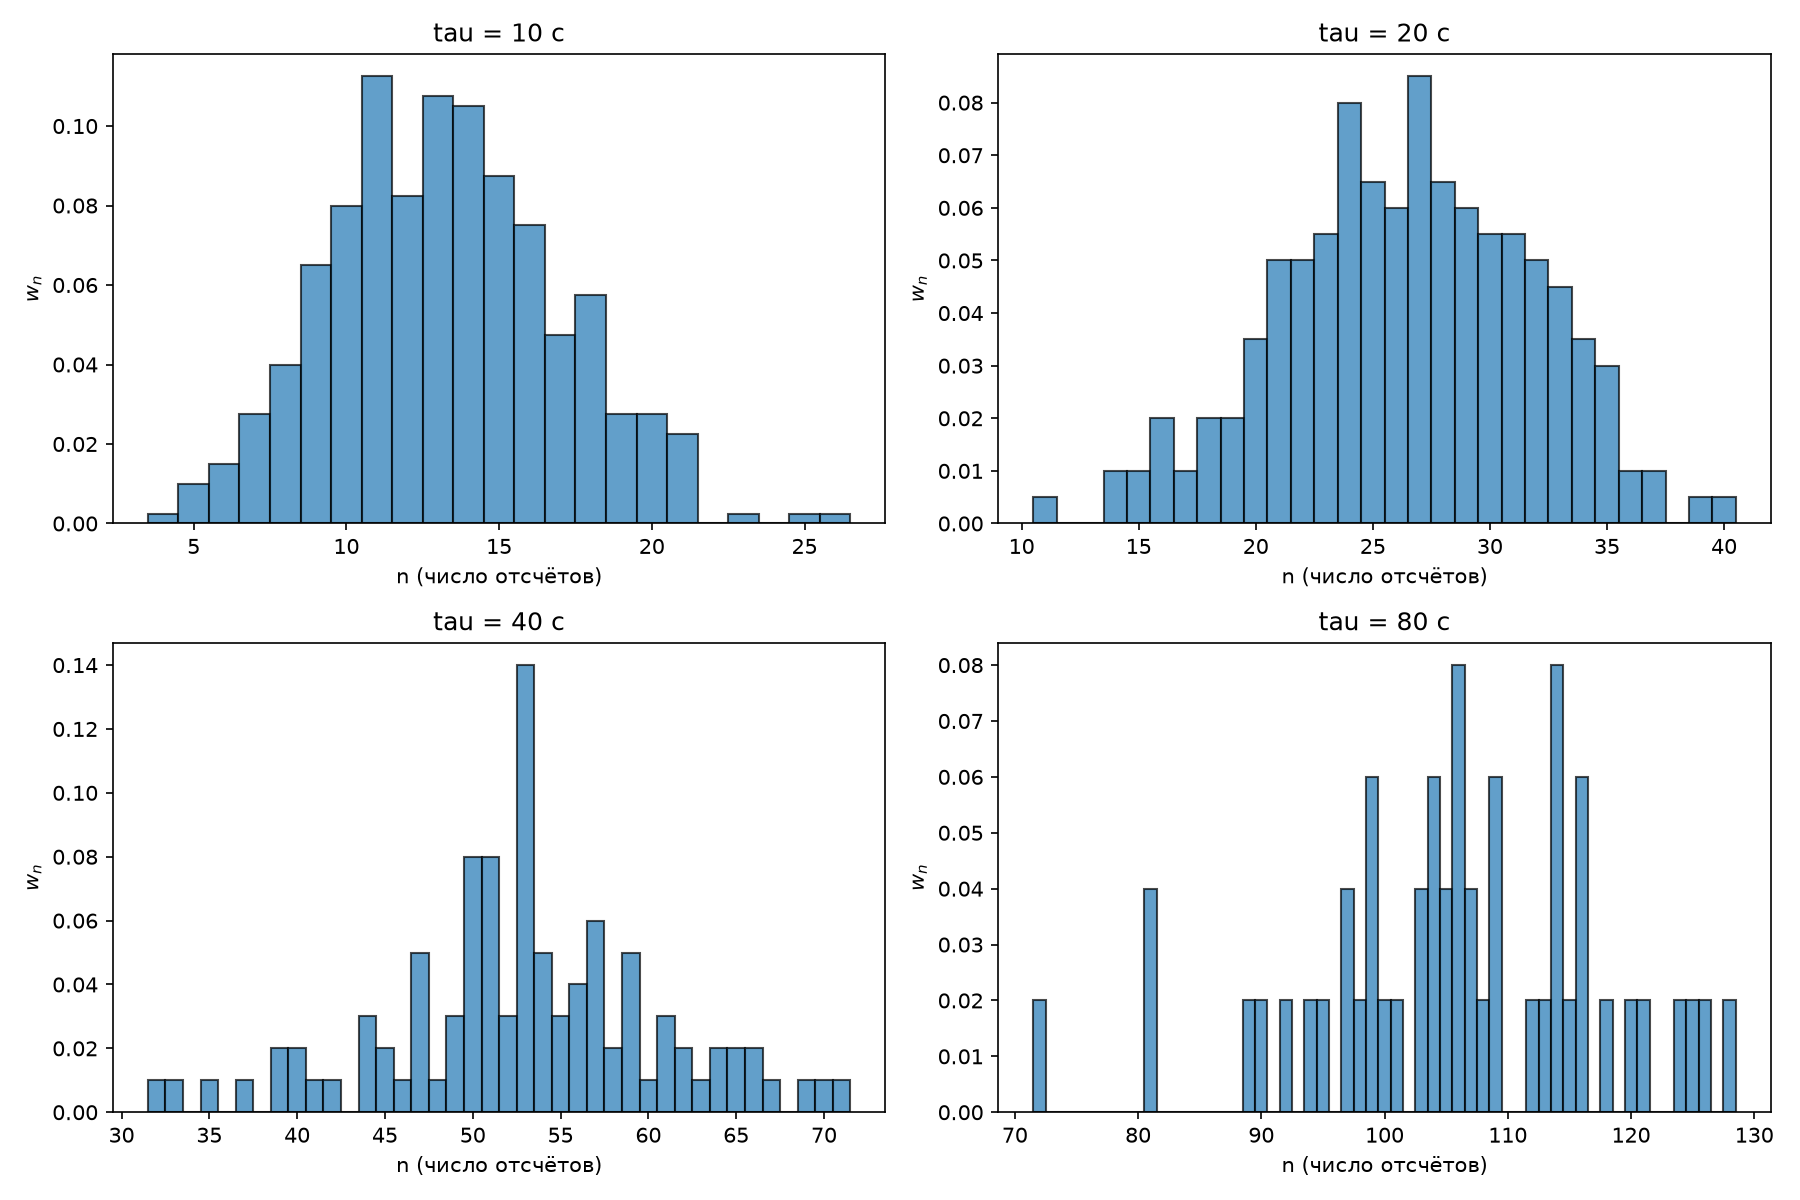
\includegraphics[width=0.9\textwidth]{histograms.png}
    \caption{Гистограммы распределения числа отсчётов счётчика для $\tau = 10, 20, 40, 80$~с}
    \label{fig:histograms}
\end{figure}

На рис.~\ref{fig:theory} экспериментальная гистограмма для $\tau=10$~с сопоставлена с теоретическими распределениями Пуассона и Гаусса, построенными по формуле~\eqref{eq:poisson} и плотности нормального распределения при параметрах $\langle n\rangle$ и $\sigma_n$, найденных из эксперимента.

\begin{figure}[H]
    \centering
    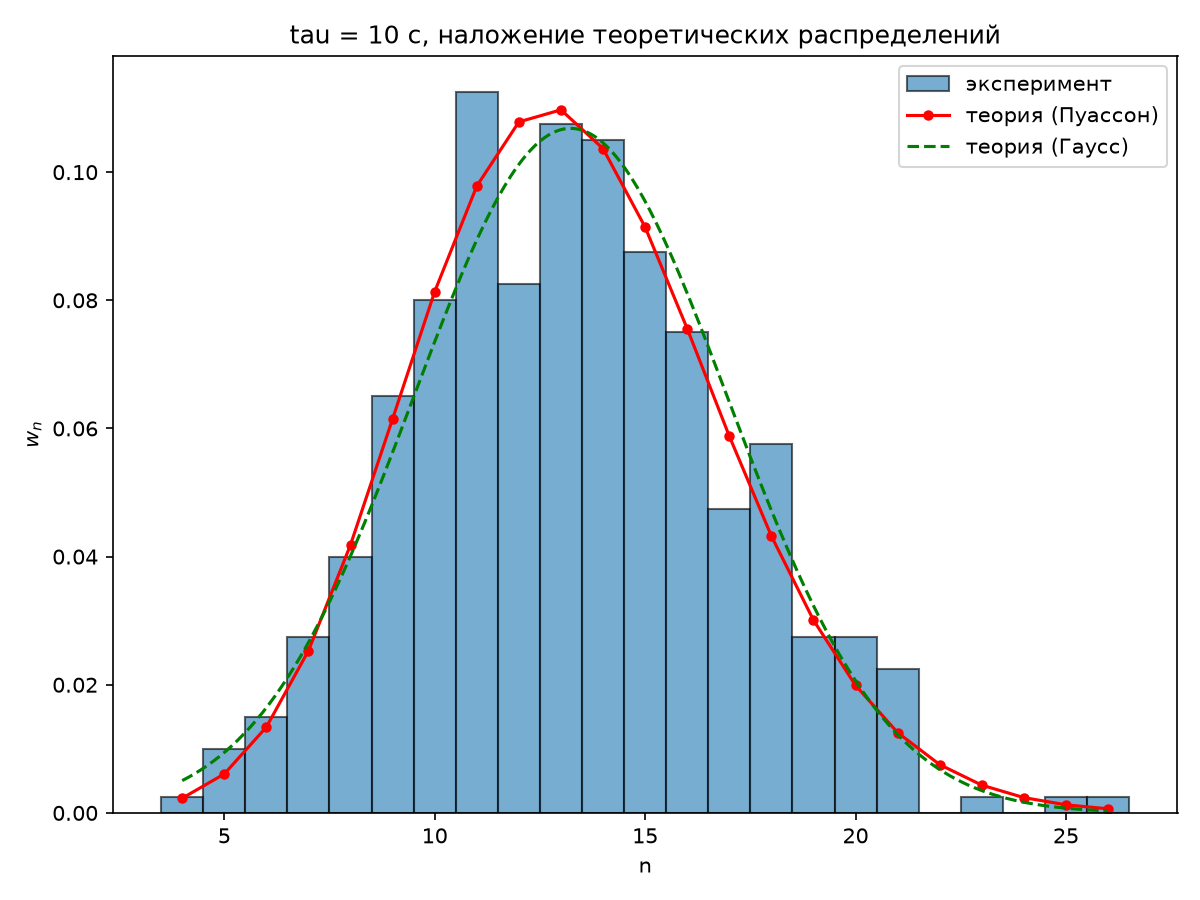
\includegraphics[width=0.7\textwidth]{histogram_theory_tau10.png}
    \caption{Сравнение экспериментальной гистограммы ($\tau=10$~с) с теоретическими распределениями Пуассона и Гаусса}
    \label{fig:theory}
\end{figure}

\subsection*{Проверка свойства распределения Пуассона}

Для каждого $\tau$ проверено выполнение равенства~\eqref{eq:poisson_property}.

\begin{table}[H]
    \centering
    \caption{Проверка свойства $\sigma_n \approx \sqrt{\langle n\rangle}$}
    \begin{tabular}{cccc}
        \toprule
        $\tau$, с & $\sigma_n$ (эксп.) & $\sqrt{\langle n\rangle}$ (теория) & расхождение, \% \\
        \midrule
        10 & & & \\
        20 & & & \\
        40 & & & \\
        80 & & & \\
        \bottomrule
    \end{tabular}
    \label{tab:poisson_check}
\end{table}

\subsection*{Доли отклонений в пределах $\sigma$, $2\sigma$, $3\sigma$}

\begin{table}[H]
    \centering
    \caption{Доли случаев в пределах $\sigma_n$, $2\sigma_n$, $3\sigma_n$}
    \begin{tabular}{ccccccc}
        \toprule
        \multirow{2}{*}{$\tau$, с} & \multicolumn{2}{c}{$|n-\langle n\rangle|\le\sigma_n$} & \multicolumn{2}{c}{$|n-\langle n\rangle|\le 2\sigma_n$} & \multicolumn{2}{c}{$|n-\langle n\rangle|\le 3\sigma_n$} \\
         & эксп., \% & теор., \% & эксп., \% & теор., \% & эксп., \% & теор., \% \\
        \midrule
        10 & & 68 & & 95 & & 99{,}7 \\
        20 & & 68 & & 95 & & 99{,}7 \\
        40 & & 68 & & 95 & & 99{,}7 \\
        80 & & 68 & & 95 & & 99{,}7 \\
        \bottomrule
    \end{tabular}
    \label{tab:sigma_intervals}
\end{table}

\section*{3. Обсуждение результатов}

\begin{itemize}
    \item Среднее число зарегистрированных частиц $\langle n\rangle$ растёт пропорционально интервалу группировки $\tau$, что соответствует постоянству средней интенсивности космического излучения.
    \item Среднеквадратичное отклонение $\sigma_n$ хорошо согласуется с теоретическим значением $\sqrt{\langle n\rangle}$, что подтверждает пуассоновский характер процесса регистрации космических частиц.
    \item Относительная погрешность определения интенсивности $\varepsilon_{\langle n\rangle}$ практически не зависит от выбора интервала группировки $\tau$ и определяется только полным числом зарегистрированных частиц за всё время эксперимента.
    \item Доли отклонений в пределах $\sigma_n$, $2\sigma_n$, $3\sigma_n$ близки к теоретическим значениям для нормального распределения, что свидетельствует о переходе распределения Пуассона к распределению Гаусса при достаточно больших $\langle n\rangle$.
\end{itemize}

\section*{Выводы}

В работе экспериментально исследована статистика регистрации фоновых космических частиц счётчиком Гейгера--Мюллера. Получено, что число отсчётов счётчика подчиняется распределению Пуассона: выполняется характерное равенство $\sigma_n\approx\sqrt{\langle n\rangle}$, а при больших средних значениях распределение хорошо описывается нормальным законом. Найдена средняя интенсивность регистрируемых частиц $j = \langle n\rangle/\tau \pm \sigma_j$ и показано, что точность её определения зависит только от полного числа зарегистрированных за весь эксперимент частиц, а не от выбора интервала группировки данных.

\section*{Список литературы}

\begin{enumerate}
    \item Попов П.В., Нозик А.А. Обработка результатов учебного эксперимента, 2019.
\end{enumerate}

\end{document}